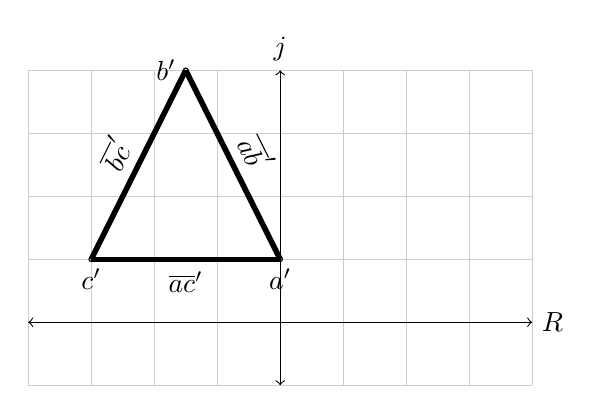
\begin{tikzpicture}[scale=0.8]
    \draw [thin,gray!40] (-4,-1) grid (4,4);
    \draw[<->] (-4,0)--(4,0) node[right] {$R$};
    \draw[<->] (0,-1)--(0,4) node[above]{$j$};
    \coordinate (1) at (0,1);
    \coordinate (2) at (-1.5,4);
    \coordinate (3) at (-3,1);
   
    \draw[black] (1) circle(1pt) node[anchor=north]{$a'$};
    \draw[black] (2) circle(1pt) node[anchor=east]{$b'$};
    \draw[black] (3) circle(1pt) node[anchor=north]{$c'$};
    \draw[line width=2pt,black,-] (1)--(2) node[midway, above, sloped]{$\overline{ab}'$};
    \draw[line width=2pt,black,-] (2)--(3) node[midway, above, sloped]{$\overline{bc}'$};
    \draw[line width=2pt,black,-] (3)--(1) node[midway, below, sloped]{$\overline{ac}'$};
\end{tikzpicture}
\caption*{Mapeo del triangulo $s$}